\documentclass[]{ccs-thesis}
% options:
% [germanthesis] - Thesis is written in German
% [plainunnumbered] - Don't print numbers on plain pages
% [earlydraft] - Settings for quick draft printouts
% [watermark] - Print current time/date at bottom of each page
% [phdthesis] - switch to PhD thesis style
% [twoside] - double sided
% [cutmargins] - text body fills complete page

% Required package
\usepackage{tikz}
\usepackage{outlines}
\usetikzlibrary{arrows,shadows} % for pgf-umlsd
\usepackage[underline=true,rounded corners=false]{pgf-umlsd}
% Protocol Header file
\usepackage{bytefield}
\usepackage{makecell}
\usepackage{tabularx}
\usepackage{tabularray}
% table coloring
\usepackage{colortbl}
\usepackage{lipsum}

\lstdefinestyle{customc}{
  belowcaptionskip=1\baselineskip,
  breaklines=true,
  frame=single,
  xleftmargin=\parindent,
  language=C++,
  showstringspaces=false,
  basicstyle=\footnotesize\ttfamily,
  keywordstyle=\bfseries\color{green!40!black},
  commentstyle=\itshape\color{purple!40!black},
  identifierstyle=\color{blue},
  stringstyle=\color{orange},
}

\lstset{escapechar=@,style=customc}

% Choose one of the following lines.
%\group{Cooperative Mobile Systems}
\group{Distributed Embedded Systems}

% Author name. Separate multiple authors with commas.
\author{Maximilian W. Gotthardt}
\birthday{13. July 1993}
\birthplace{Berlin}

% Title of your thesis.
\title{Evaluation of protocols for control stage lighting}

% Degree program.
\thesistype{Bachelor Thesis in Computer Engineering}\thesiscite{Bachelor Thesis~(Bachelorarbeit)}

% List of advisors, separated by commas. Delete if identical to referees or inapplicable.
\advisors{Anatolij Zubow}

% List of referees, separated by commas.
\referees{Falko Dressler, Thomas Sikora}

% Abbreviations own
\acrodef{RR}{Rapid Repetition}
\acrodef{MCU}{Microcontroller Unit}

% Abbreviations light protocols
\acrodef{DMX}{Digital Multiplex}
\acrodef{CANhashing}[CAN]{Content Addressable Network}{extra={when referring to the distributed hash table}}
\acrodef{CANproto}[CAN]{Controller Area Network}{extra={when referring to the bus protocol}}

% Abbreviations Networking
\acrodef{UDP}{User Datagram Protocol}
\acrodef{OSI}{Open Systems Interconnection}
\acrodef{MAC}{Media Access Control}
\acrodef{DL}{Data Link}
\acrodef{IP}{Internet Protocol}
\acrodef{IEEE}{Institut of Electrical and Electronics Engineers}
\acrodef{CD}{Collision Detection}
\acrodef{CSMA/CA}{Carrier-sense multiple access with collision avoidance}
\acrodef{DCF}{Distributed Coordination Function}
\acrodef{PCF}{Point Coordination Function}
\acrodef{DIFS}{DCF Inter Frame Spaces}
\acrodef{SIFS}{Short Inter Frame Spaces}
\acrodef{NAV}{Network Allocation Vector}
\acrodef{PHY}{Physical Network Layer}
\acrodef{CW}{Contention Window}
\acrodef{MPDU}{}
\acrodef{DSSS}{Direct Sequence Spread Spectrum}
\acrodef{FHSS}{Frequency Hopping Spread Spectrum}
\acrodef{STA}{Station}
\acrodef{AP}{Access Point}
\acrodef{WES}{Wireless Endsystem}
\acrodef{BSS}{Basic Service Set}
\acrodef{OFDM}{Orthogonal Frequency Division Multiplexing)}
\acrodef{MIMO}{Multiple Input-Multiple Output)}
\acrodef{WLAN}{Wireless Local Area Network}

\begin{document}

\pagenumbering{roman}

\maketitle

\thispagestyle{empty}

\cleardoublepage

\chapter*{Abstract}
\addcontentsline{toc}{chapter}{Abstract}
\begin{otherlanguage*}{american}

about 1/2 page:
\begin{enumerate}
	\item Motivation (Why do I care?)
	\item Problem statement (What problem are I trying to solve?)
	\item Approach (How did I go about it)
	\item Results (What's the answer?)
	\item Conclusion (What are the implications of the answer?)
\end{enumerate}
	

In the field of lighting and stage technology, the challenge of controlling the individual installations, called 'fixtures', quickly and without complications is a recurring one. Established solutions are realized via cables. 

However, due to the progress in radio technology, wireless solutions are becoming more and more common. Therefor is often expensive hardware needed.
Parallel to this there is a fast growing market around creative and individually developed DIY projects, which have found their own niche. Durch niedrigpreisige 
While most commercial solutions still rely on expensive and complex wired control, it is particularly suitable for smaller projects to experiment with the new wireless technologies. 
In this thesis I try to implement a wireless solution, which does not need an IP-Layer using the popular platform ESP and the properitary protocol ESP-NOW to distribute the light information to each fixture. 
ESP-Now instead works more like an direct radio communication.
	
\end{otherlanguage*}

\chapter*{Kurzfassung}
\addcontentsline{toc}{chapter}{Kurzfassung}
\begin{otherlanguage*}{ngerman}
\begin{itemize}
	\item kabellose lösungen werden interessant
	\item chips werden günstiger
	\item für kleine projekte leider sehr teuere Hardware
	\item 802.11 wird als standard benutzt
	\item protokolle wie art-net könnten optimiert werden
	\item esp plattform bietet interssante möglichkeiten, wegen der geringen kosten der chips und esp-now
	\item entwicklung einer plattform die esp-now nutzt
	\item verschiedene ansätze studiert, wie broadcast und unicasts
	\item mit jeweils unterschiedlichen modifikationen
\end{itemize}


\end{otherlanguage*}
\acresetall

\cleardoublepage
\tableofcontents
\TODO{The table of contents should fit on one page. When in doubt, adjust the \texttt{tocdepth} counter.}

\cleardoublepage
\pagenumbering{arabic}



\chapter{Introduction}
%\chapter{Einleitung}

\begin{itemize}
\item general motivation for your work, context and goals.
\item context: make sure to link where your work fits in
\item problem: gap in knowledge, too expensive, too slow, a deficiency, superseded technology
\item strategy: the way you will address the problem
\item recommended length: 1-2 pages.
\end{itemize}

In the subject area 

====

In the field of lighting and stage technology, the challenge of controlling the individual installations, called 'fixtures', quickly and without complications is a recurring one. 
Established solutions are realized via cables.

\section{Motivation/Requirements}
\begin{itemize}
\item Reliability
\item .. and why 100\% Reliability is not important (pyrotechnics)
\item Lower latency
\item Synchronisation
\item higher update frequency
\item Range
\end{itemize}

\section{Challenges}
\begin{itemize}
\item low cost
\item (ESP Platform)
\item DIY community
\end{itemize}

\section{Problemstatement and Contribution WICHTIG}
\begin{itemize}
\item open source available on github [link]
\item thought-provoking impulse for different approaches
\item Protocol auf DL Layer/App Layer Ebene
\item Art-Net baseline
\item simulativ und experimentel untersucht
\end{itemize}

\section{Thesis Outline}
\begin{itemize}
	\item A First Implementation and Evaluation of the IEEE 802.11aa Group Addressed Transmission Service    
		\subitem unsosliced Repetition
		\subitem blockack
	\item Evaluation of Error Control Mechanisms for 802.11b Multicast Transmissions
		\subitem packet loss rate
		\subitem ARQ, FEC
	\item ESP-NOW communication protocol with ESP32
		\subitem ESP-NOW details
	\item The Working Principles of ESP32 and Analytical Comparision of using Low-Cost Microcontroller Modules in Embedded Systems Design
		\subitem why the ESP32 is superior over arduino
	\item Adaptive Cross-Layer Protection Strategies for Robust Scqalable Video Transmissions Over 802.11 WLANs
	\item Voice Capacity of IEEE 802.11b, 802.11a and 802.11g Wireless LANs
\end{itemize}

\clearpage
\section{References}

What follows is just a very quick refresher on how to use references.
It is not a guide on scientific writing in general, nor copyright and plagiarism in particular.
Please refer to an actual guide on technical writing and scientific practices to make sure you understand how, where, and when to cite.

Simply speaking, proper scientific writing has to deal with two closely related (but not identical) concepts:
\begin{enumerate}[label=\alph*),ref=(\alph*)]
\item\label{itm:ref:copy}
Copyright
\item
Plagiarism\label{itm:ref:plag}
\end{enumerate}
Do not confuse the need for properly citing your sources as something related to copyright.
Questions of~\ref{itm:ref:copy} copyright or the corresponding national equivalent deal with who has the right to reproduce a certain text excerpt, an image, or something similar.
Questions of~\ref{itm:ref:plag} plagiarism deal with who came up with a certain idea or insight, e.g., a certain finding, a certain concept, or a certain way of illustrating a concept.
By way of analogy, consider a car: after buying a car you have the right to~\ref{itm:ref:copy} do whatever you want with it, but you still cannot claim that you~\ref{itm:ref:plag} invented it.
Conversely, properly~\ref{itm:ref:plag} crediting who invented your neighbor's car does not give you the right to~\ref{itm:ref:copy} use it.
Put yet another way, problem~\ref{itm:ref:copy} is a legal one: to be allowed to publish a scientific work you (or, rather, your publisher) needs to have permission to reproduce it -- or suffer legal consequences like heavy fines.
Problem~\ref{itm:ref:plag} is an academic one: claiming someone else's ideas as one's own is plagiarism; similarly, re-selling old ideas as new ones is self-plagiarism.
Both incur heavy penalties like exclusion from schools and professional associations or being blacklisted from publishing with scientific outlets for any number of years.

You will need to address both problems in writing your thesis.
Problem~\ref{itm:ref:copy} can be addressed in two ways:
First, by creating original content (that is, text or figures) yourself, which is always preferable as this gives you the freedom to present the content your way.
Second, by obtaining a license to reproduce content (e.g., by way of buying a license or adhering to the terms of an existing copyleft license).
Problem~\ref{itm:ref:plag} can be addressed in two ways:
First, presenting original ideas and insights (as you will do when presenting own results).
Second, by clearly pointing out the (primary) source of an idea.
The latter is the topic of this section.

In brief, use references whenever you cite from related work (either directly or indirectly), or when you build on related work (this includes their way of illustrating a particular concepts, in text form as well as in the overall design of a figure).
Also use references to point a reader to related work.
Clearly distinguish between these uses.
Make it very clear which part of a statement a reference belongs to.
Compare the following three, vastly different uses (where the cited idea appears in \textbf{boldface}):

\begin{itemize}
\item ``\textbf{Foo and bar are of equal value. Thus, any can be used.}''~\cite{akyildiz2002survey,arampatzis2005survey}
\item According to~\cite{akyildiz2002survey} and~\cite{arampatzis2005survey}, \textbf{foo and bar are of equal value, and any can be used}.
\end{itemize}
versus
\begin{itemize}
\item ``\textbf{Foo and bar are of equal value}''~\cite{akyildiz2002survey,arampatzis2005survey}. Thus, any can be used.
\item According to~\cite{akyildiz2002survey} and~\cite{arampatzis2005survey}, \textbf{foo and bar are of equal value}. From this it follows that any can be used.
\end{itemize}
versus
\begin{itemize}
\item Foo and \textbf{bar}~\cite{akyildiz2002survey,arampatzis2005survey} are of equal value. Thus, any can be used.
\item Foo and \textbf{bar} (detailed in~\cite{akyildiz2002survey} and~\cite{arampatzis2005survey}) are of equal value. Thus, any can be used.
\end{itemize}
versus
\begin{itemize}
\item \textbf{Foo}~\cite{akyildiz2002survey} and \textbf{bar}~\cite{arampatzis2005survey} are of equal value. Thus, any can be used.
\item \textbf{Foo} (detailed in~\cite{akyildiz2002survey}) and \textbf{bar} (detailed in~\cite{arampatzis2005survey}) are of equal value. Thus, any can be used.
\end{itemize}

Never typeset a reference after the final full stop of a paragraph (or sentence) and expect your reader to figure out which part of the paragraph is an indirect citation and which part is original (i.e., your own) work.
When paraphrasing longer passages of text, use an indirect citation.
Make sure to clearly point out when you are finished paraphrasing, like so:
\emph{According to \textcite{akyildiz2002survey}, Foo and Bar can be characterized as follows. They are big. They are bright. The authors further argue that one can be substituted for the other. In the following I will go on to prove that this is not true.}

When citing more than a few pages worth of text, point the reader to the specific part you are referring to in your citation, like so:
\emph{In recent years, an increasing number of cyclists are switching from air filled tires to cement filled ones~\cite[Table IV]{dietrich2009lifetime}}.

If a figure or a table is closely based on another one, make sure to cite its source, preferably in its caption, like so:
\emph{Figure 1 -- the relation of ravens and writing desks (based on~\cite[Figure~42]{dietrich2009lifetime})}.
Be aware that, while there is a well-established convention on how to illustrate a verbatim quote of text (by using quotation marks), there is no well-established convention for indicating that an image was copied verbatim.
Thus, when citing a figure or table, you must explicitly state whether it was copied verbatim, ed, or whether it served as inspiration for your own.

Do not cite URLs. Content found there is not peer reviewed and it is likely to change during the lifetime of your work.
For pointing a reader to interesting websites, use footnotes -- but trust your reader to know how to use a web search engine.

Your text reads nicer if you do not use citations as a substitute for nouns (like this section did).
Instead of \emph{The benefits of cement filled tires has been shown by \cite{akyildiz2002survey}}, consider writing \emph{\textcite{akyildiz2002survey} have shown the benefits of cement filled tires}.
The \texttt{textcite} command makes this straightforward.

Make sure to read your bibliography section (that is, the typeset list of references) after you are done adding all citations to your text.
Does it contain all information needed to uniquely identify to references you used?
Do not trust BibTeX files you find on the web:
Digital libraries frequently have their contents wrong, are missing information, or are using different field names than your bibliography style expects (leading to missing information in the typeset bibliography).
To give a few examples:
Check the authors' list (making sure all authors are listed in the same order and in the same way they are listed in the publication).
Check the conference location (it's most likely not ``New York, New York'').
Check the publisher name (many digital libraries use a field that is not typeset by your bibliography style; have a look at the demo bibliography in this template for how to deal with that).
Check the page numbers (many digital libraries put ``1--5'' here despite the paper starting at a later page -- or despite it not having any page numbers to begin with).
Check the conference name, put its parts in a logical order, and lose the ``in proceedings of'' (it's not ``Mobicom, in proceedings of, 1999 series MobiCom99'' but ``5th ACM International Conference on Mobile Computing and Networking (MobiCom 1999)''.\todo{triple-check all references}

\chapter{Related Work}
\begin{itemize}
	\item Wie der und der in Paper so gezeigt hat 
	\item Auch Ding et al haben versucht
	\item ...
	\item 10 Paper
	\item halbe seite
\end{itemize}

Foo and bar~\cite{LowCostMicrocontroller} are of equal value. Thus, any can be used.\\
According to~\cite{akyildiz2002survey}

Wireless solutions for stage lighting are growing fast. 


\chapter{Fundamentals}
\label{sec:fundamentals}

\begin{itemize}
	\item describe methods and techniques that build the basis of your work
	\todo{don't get what methods and techniques i was using}
	\item include what's needed to understand your work (e.g., techniques, protocols, models, hardware, software, ...)
	\item exclude what's not (e.g., anything you yourself did, anything your reader can be expected to know, ...)
	\item review related work(!)
	\todo{List of papers:}
	\item recommended length: approximately one third of the thesis.
\end{itemize}

In this chapter the fundamentals required for understanding the different approaches 
in this thesis using are explained.
This contains basic knowledge of the physical- and data link layer,
which are located in the first and second layer of the \ac{OSI} Model.\todo{refrence to table below}.\\
% alternativ introduction
In order to understand the upcomming ESP-Now protocol we have to take a look at the \ac{DL} layer in 802.11.
It is the second layer of the \ac{OSI} model of computer networking illustrated in \cref{tab:OsiModel}.
\TODO{Rewrite introduction in chapter Fundamentals!}

\begin{table}
	\centering
	% \label{tab:layer_overview}
	\begin{tabular}{ |c| } 
		\hline
		Application layer\\
		\hline
		Presentation layer\\
		\hline
		Session layer\\
		\hline
		Network layer\\
		\hline
		\cellcolor{yellow!25}Data Link layer\\
		\hline
		\cellcolor{yellow!25}Physical layer\\
		\hline
	\end{tabular}
	\caption{\ac{OSI} model}
	\label{tab:OsiModel}
\end{table}

\section{IEEE 802.11 Specification Family}

The \ac{IEEE} 802 is a family of standards dealing with area networks different kinds.
\begin{itemize}
	\item 802.11 \ac{WLAN}
	\item 802.15.1 Wireless Personal Area Network (WPAN)
	\item 802.15.4 Low-rate WPAN (LR-WPAN)
	\item 802.16 Wireless metropolitan area network (WMAN)
\end{itemize}

For this thesis is the focus set to the 802.11, because of the accessability and wide functionality.
There are two \ac{BSS} defined:
\begin{itemize}
	\item Infrastructure BSS\\
	A central element manages the network and all the traffic goes through. 
	Every \ac{STA} must always communicate via the \ac{AP} and never directly - exceptional: Direct Link Mode.
	An initial association must take place to use this \ac{BSS}.
	This is the most common mode a \ac{WLAN} is used.
	\item Independent BSS\\
	A network without a central station, where the network topology can flexible change over time.
	The communication happens directly between the Wireless Endsystems.\todo{WES in AdHoc correct?}
	Efficent routing can became a problem in more complex topologys.
\end{itemize}
The most common use in 802.11 is the Infrastructure mode.\\ 

\subsection{IEEE Frame Structure}
• Image of 802.11 frame structure PHY and MAC header\\
• Image of MAC header\\
• Image of frame control field of MAC in MAC header\\
• Image of frame control field of MAC in MAC header\\

\begin{figure}
	\centering
	\begin{bytefield}[bitwidth=1.1em, bitheight=\widthof{~Duration~}, boxformatting={\centering\small}]{29}
		\bitheader[endianness=little]{0-29} \\
		\bitbox{2}{FC} &
		\bitbox{2}{\rotatebox{90}{Duration}} &
		\bitbox{6}{Address\\1} &
		\bitbox{6}{Address\\2} &
		\bitbox{6}{Address\\3} &
		\bitbox{2}{SC} &
		\bitbox{6}{Address\\4}
	\end{bytefield}
	\caption{MAC header in a WLAN frame}%
	\label{fig:mac_header}%
\end{figure}

802.11ac and later using frame aggregation in order to reduce overhead.

\subsection{Physical layer}
There are several complements to the 802.11 standard.
\begin{itemize}
	\item 802.11b \\
	supports larger bitrates with \ac{DSSS} or \ac{FHSS} as modulation from 1Mbit/s to 11Mbit/s.
	It uses the 2.4 GHz ISM band.
	\item 802.11a and 802.11g \\
	with \ac{OFDM} data rates are increased up to 54 Mbit/s.
	Where 802.11a is in the 5GHz ISM band 802.11g uses the 2.4GHz ISM band.
	\item 802.11n\\
	It also uses \ac{OFDM} and improves with additionaly \ac{MIMO}, channel bonding and frame aggregation to increase the bandwidth and decrease the overhead.
	Using 2.4 GHz and 5GHz ISM band.
	\item 802.11ac\\
	Support of wider channel and out of it higher bitrates. It also includes features like Multi-User MIMO.
	It only uses the 5 GHz ISM band.
	\item 802.11ax\\
	Like 802.11ac but with additional use of the 6GHz ISM band and better power control. 
	Also called WiFi6.
\end{itemize}

\subsection{DL-Layer in 802.11}

\begin{itemize}
	\item why is it important for us
	\item how works the DL layer
	\item was ist BC, was Unicast
	\item was sind frames
	\item how the Application layer
\end{itemize}

\subsubsection{Unicast}

The link layer unicast is used to send data over an single hop to the target \ac{WES} destination.
The link layer of each \ac{WES} checks the destination MAC address in the link layer header and discards the frame if the destinatin address does not match its own address.\\

Unicast is by default reliable.

E.g. the \ac{AP} wants to transmit a packet to one specific \ac{WES}\\
When the Unicast reaches the destination \ac{WES} an acknowledgement frame is send back after the \ac{SIFS} + backoff.\todo{when to explain CSMA/DC?}

If the acknowledgement is not successfully received by the sender, the sender will repeat the transmission for a given number.
When the number is exceeded, the packet could not be delivered. 
If the number is set to zero, the unicast can be considered as non-reliable.
\TODO{example}

\todo{complete figure UC}
\begin{figure}[h]
	\centering
	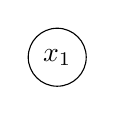
\begin{tikzpicture}[main/.style = {draw, circle}] 
		\node[main] (1) {$x_1$}; 
	\end{tikzpicture} 
	\caption{Unicast Transmission}
	\label{fig:unicast_topology}
\end{figure}

\subsubsection{Broadcast}

If a packet should be received from all \ac{WES}'s it can be distributed as broadcast.
The \ac{MAC} address of the destination address in the link layer is set to the common broadcast address, which is ff:ff:ff:ff:ff:ff.\\
In contrast to unicast, broadcast is not reliable. 
This is mainly because the packet is addressed to all nodes at the same time, and if link layer acknoledgements would be used, 
the acknoledgements would be sent by all nodes at the same time, 
because there is no mechanism in which order acknoledges should be answered. 
In addition, the sender of a broadcast does not know how many WESs he is addressing the packet to in the first place.
Retransmitting acknoledgements would lead to massive collision and loss of acknoledgements.
E.g. management information in a \ac{WLAN} is sent in a broadcast mode, because it has to reach every \ac{WES} and isn't worth to be acknoleged.

\todo{complete figure BC}
\begin{figure}[h]
	\centering
	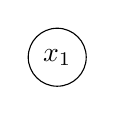
\begin{tikzpicture}[main/.style = {draw, circle}] 
		\node[main] (1) {$x_1$}; 
	\end{tikzpicture} 
	\caption{Broadcast Transmission}
	\label{fig:broadcast_topology}
\end{figure}


\subsection{Multicast}

\TODO{Mutlicast explain multicast mac address}
When the same packet should be transmitted to multiple \ac{WES}'s, but not to all, multicast can be used.
Transmitting the same packet multiple times via unicast is wasteful.
There are different approaches to realize acknowledgements for mutlicasts.
They differ mainly by the respective field of application.
\TODO{example}
Link layer multicast is often used for large files in audio or video streams, where a big amount of data is distributed and multiple clients listen simultaneously.

\todo{complete figure UC}
\begin{figure}[h]
	\centering
	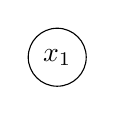
\begin{tikzpicture}[main/.style = {draw, circle}] 
		\node[main] (1) {$x_1$}; 
	\end{tikzpicture} 
	\caption{Multicast Transmission}
	\label{fig:multicast_topology}
\end{figure}

\subsection{IEEE 802 Stuff}
Multiple Access/Multiplexing: When Signals to/from different users share a common channel using time division methods (TDM/TDMA, CSMA)\todo{eigene Worte}\\

DSSS: Usage of multiple antennas
(up to 4) to increase data rates\\

Addressing
In a LAN environment, devices are logically separated using 48-bit
globally unique MAC addresses: example
In IPv4 networks (e.g. Internet), nodes are logically separated
using 32-bit globally unique IP addresses: example \\

Routing
• Routing in a (W)LAN is based on MAC addresses, never IP addresses.\\
• A router (e.g. integrated with an access point) performs mapping between\\
these two address types: \\

Address allocation
• MAC addresses are associated with the hardware devices.\\
• IP addresses can be allocated to (W)LAN devices either on a\\
permanent basis or dynamically from an address pool using the
Dynamic Host Configuration Protocol (DHCP). \\

Mesh networks
are able to relay frames from one device to another.
• Provide coverage extension over multiple hops (e.g. Internet access)
• Sufficient address information is required to be able to relay data from a
source device to the ultimate destination (IP or MAC address).
This can be used to extend the range from on \ac{WES} to another \ac{WES} over some other \ac{WES}.
Since range isn't a critical parameter in this thesis, it hasn't to be further discussed.\\

Beacon Frames
contain the channel information found during passive scanning. Probe request are used in acting scanning.\\

Backoff: 
random time delay to avoid collisions\\

DIFS/SIFS:
Delay between transmissions used for \ac{CSMA/CA}

\section{ESP Platform}
\begin{itemize}
	\item Why ESP Platform 
	\item whats is the alternative
	\item chip shortage for Arduino
	\item price gab to esp32 dev boards
\end{itemize}
Almost every 802.11 capable \ac{MCU} could be picked for this research.
But there are several reasons why the ESP Platform from Espressif is a valid choice.
There are several chips provided by Espressif with WiFi specifications, these chips are very affordable (\todo{ESP32 Kosten in € 2021 aufführen? Link? Datum?}) 
and althrough the ongoing chip crysis (2021) there are easy to get, in contrast of the also very popular Chips from the manufacturer Arduino, which are also more expansive.
Espressif supports an own development IDF to flash the chips, with minor tweeks it's also to use the Arduino IDE.\\
However the properitary protocol ESP-Now which, just supported in the ESP Platform is discussed below \cref{sub:ESP-Now} has promising properties for the realisation of a low level protocol.

\section{Light protocols}

In this chapter I give you a short introduction about stage lighting protocols that are already in use. 
After that I will discuss why I choosed the ESP Platform and which modifications I made to get the improvements I was looking for in the requirements.
\todo{use passive voice} 

\subsection*{DMX-512A}
\ac{DMX}, is the current industry standard for stage lighting. It is based on \ac{CANproto}, therefore it uses wires.

All devices, called fixtures, are daisy chained together.
\TODO{Picture of topology}

% \subsubsection{fixture}
A fixture is a lighting instrument, 
this could be a moving-head, fresnel, spotlight, stroboscope or any other light installation.
It could also be a fog machine that emits fog on an appropriate signal.
Since \ac{DMX} is unidirectional we \todo{I or we? It should be I...} can assume that fixtures generally only receive or forward (daisy chain) control signals sent from the control console.
In this thesis I equate it with a node or an entity receiving a signal.
\TODO{Show Hardware e.g. DMX Plug}

% \subsubsection*{Channel}
A channel in the event technology is to distinguish between e.g. a WiFi channel. 

Each FIXTURE is assigned at least one, but usually several CHANNEL, which are the payload containing in a packet to all FIXTURES. 
Each fixture knows which CHANNEL is intended for it. Each channel consists of one byte.
For example, an RGB LED spotlight could have three channels, one for each color.
Due to the resolution of one byte, the individual colors can (theoretically) be controlled in 256 different intensities.
\TODO{Bild von fixtures verteilt auf channel}

% \subsubsection*{DMX-Universe}
A universe can contain a set of 512 Channel. If there is a need of more channels one needs more DMX universes.
Due to the fact that a DMX universe always has its own bus, starting from its own controller, this can lead to inconveniences.

\subsection{Art-Net}
\label{sec:artnet}
\begin{itemize}
\item 2.4 or 5GHz
\item DMX-Like
\item related work
\end{itemize}

Due the limitation of 512 channel for each universe there where protocols implemented using the 
Art-Net also called Art-Net DMX is 

\subsection{ESP32 Hardware}
\begin{itemize}
\item reasons to pick
\item availability due chipcrysis
\item cheap chip
\item Range
\item Properity
\item Reverse-Engineering 
\item related work
\item 2.4 GHz (cheap)
\item Bild vom chip
\end{itemize}
The chip ESP32 is quite common in DIY projects around everything from home automation to light installations. The chip supports the 

\subsection{ESP-Now}
\label{sub:ESP-Now}
\begin{itemize}
\item How does ESP-Now match the requirements from the motivation
\item 250 payload
\item gaps in the documentation
\end{itemize}

ESP-NOW is a properitary protocol developed by Espressif. 
ESP-NOW is widely used in smart light, remote controlling, sensor, etc.\todo{cite ESP documentation website}. 
It is a conectionless protocol, so the \ac{WES}'s' are in Ad-Hoc mode insted of \ac{STA}.
It is just supported with the ESP8266, ESP32 and ESP32, these are all chipsets from Espressif, but they are compatible with each other.
Because of this, a ESP-Chip as gateway is needed to interact from the outside to the ESP-NOW network. 

Through the hardware limitation of the boards it can just be used on the 2.4 GHz frequncy band.
ESP-NOW allows 10 ESPs for pairing with encryption and up to 20 without encryption.
Espressif promises throuput of up to 30MBit/s with UDP transmissions over the air and a possible range of up to 1km.
However \emph{\textcite{ESPNOWPaper}} measured a range of the unmodified onboard antenna of the ESP32 
and just got a \emph{\textcite{ESPNOWPaper} stable commication up to 190m in open field}.\\

The ESP-NOW protocol has a focus on low power consumption.
A connectionless communication between \ac{WES}'s not only saves energy during the authentication process, 
Additionally, is the commonication the the properties of the ad-hoc mode, direct and not over a second access point.
The protocol has a limitation of a limeted payload of 250 byte for each transmission.
It also has a much less overhead, which results in shorter airtime, less disturbances and also less power consumption through the antenna 
(latter is not relevant for this thesis).
There is no TCP/IP header to be transmited. 
For very small payloads, this offset can become dispropotional.

The default ESP-NOW bit rate is 1 Mbps it uses a channelwidth of 20MHz, there is no double channel (40Mbit/s or higher) used.
But e.g. the low energy, high range protocol Long Range Wide Area Network (LoRaWAN) suffers from a to slow throuput for this application.

To undersant what ESP-NOW does it needs to take a look to the vendor-specific action frame transmiting ESP-NOW data. 
\todo{cite somehow the ESP-NOW documentation pdf: ESP-IDF Programming Guide: ESP-NOW, source: \url{https://docs.espressif.com/projects/esp-idf/en/latest/esp32/api-reference/network/esp_now.html}}

% \url{https://www.heise.de/tipps-tricks/}

visualized in \ref{fig:esp-now_frame_format}.

\begin{table}[h]
	\centering
	\begin{tblr}{	hlines,
					vlines,
					rows = {ht=1.3cm},
					columns = {halign=c},
					colspec = {XXXXXX},} 
	\makecell{MAC\\Header}& \makecell{Category\\Code} & \makecell{Org.} & \makecell{Random\\Values} & \makecell{Vendor\\Specific\\Content} & \makecell{FCS} \\
	\end{tblr}
	\begin{tabularx}{\linewidth}{ X X X X X X }
		\makecell{\footnotesize{24}} & \makecell{\footnotesize{1}} & \makecell{\footnotesize{3}} & \makecell{\footnotesize{4}} & \makecell{\footnotesize{7 $\sim$ 255}} & \makecell{\footnotesize{4}} \\
	\end{tabularx}
	\caption{ESP-NOW Frame Format}
	\label{fig:esp-now_frame_format}
\end{table}

\begin{itemize}
	\setlength\itemsep{-0.5em}
	\item \textbf{MAC Header:} As ESP-NOW is connectionless, the MAC header differs from that of standard frames.
	\item \textbf{Category Code:} The Category Code field is set to the value(127) indicating the vendor-specific category.
	\item \textbf{Organization Identifier:} The Organization Identifier contains a unique identifier (0x18fe34), which is the first three bytes of MAC address applied by Espressif.
	\item \textbf{Random Value:} The Random Value filed is used to prevents relay attacks.
	\item \textbf{Vendor Specific Content:} The Vendor Specific Content contains vendor-specific fields (table \ref{fig:esp_now_vendor_format})
	\item \textbf{Frame Check Sequence:} Used for error correction in layer 2.
\end{itemize}

Inside of the ESP-NOW frame \ref{fig:esp-now_frame_format} is the vendor specific content visualized in \ref{fig:esp_now_vendor_format}. 

\begin{table}[h]
	\begin{tblr}{	hlines,
					vlines,
					rows = {ht=1.3cm},
					columns = {halign=c},
					colspec = {XXXXXX},} 
		\makecell{Element\\ID}& \makecell{Length} & \makecell{Org.\\Identifier} & \makecell{Type} & \makecell{Version} & \makecell{Body}  \\
	\end{tblr}
	\begin{tabularx}{\linewidth}{ X X X X X X }
		\makecell{\footnotesize{1}} & \makecell{\footnotesize{1}} & \makecell{\footnotesize{3}} & \makecell{\footnotesize{1}} & \makecell{\footnotesize{4}} & \makecell{\footnotesize{7 $\sim$ 250}} \\
	\end{tabularx}

	\caption{Vendor Specific Action Frame}
	\label{fig:esp_now_vendor_format}
\end{table} 

\begin{itemize}
	\setlength\itemsep{-0.5em}
	\item \textbf{Element ID:} The Element ID field is set to the value (221), indicating the vendor-specific element.
	\item \textbf{Length:} The length is the total length of Organization Identifier, Type, Version and Body.
	\item \textbf{Organization Identifier:} The Organization Identifier contains a unique identifier(0x18fe34), which is the first three bytes of MAC address applied by Espressif.
	\item \textbf{Type:} The Type field is set to the value (4) indicating ESP-NOW.
	\item \textbf{Version:} The Version field is set to the version of ESP-NOW.
	\item \textbf{Body:} The Body contains the ESP-NOW data.
	\todo{this is cited from espressif manual!!}
\end{itemize}

It is worth to mention, that the vendor specific content \ref{fig:esp-now_frame_format} is allowed to contain up to 255 byte,
but the sum over all values in \ref{fig:esp_now_vendor_format} if the body would contain the maximum of 250 bytes, 
leads to a total of 260 bytes.
The values are from the documentation of ESP-NOW from Espressif.
They also claim, that broadcast is not supported in ESP-NOW, but it is.
It seems that the documentation isn't complitly finished (or translated).

\subsection{ESP-Now vs Art-Net Baseline}
\todo{subsection can be on a wrong position!}
\TODO{remove newpage command}
\begin{itemize}
	\item Network stack diagram
	\item baseline
\end{itemize}

\lipsum[1]

\chapter{Proposed Approach}
\begin{itemize}
\item describe everything you yourself did (as opposed to the fundamentals chapter, which explains what you built on)
\item start with a theoretical approach
\item describe the developed system/algorithm/method from a high-level point of view
\item go ahead in presenting your developments in more detail
\item recommended length: approximately one third of the thesis.
\end{itemize}

Starting from the ESP-Now protocol, different approaches can be chosen to route the control signals to the fixtures. 
In the following I will present different approaches, which are also investigated experimentally.

\section{Design}
\label{sec:design}
\begin{itemize}
	\item Specification of the protocols
	\item analytic results (simulierte Ergebnisse)
	\item Ad-Hoc complexity of topology is not a problem, because of its simple star structure.
\end{itemize}

In this chapter there are different approaches presented and discussed.
There are several specifications to go through and some details of the implementation.

\subsection{Slim Unicast}
\begin{itemize}
\item topology
\item Network stack
\item re transmissions
\item reliability
\item tolja calculation sheet for 802.11
\item wireshark measurements
\end{itemize}

Art-Net \cref{sec:artnet} makes use of the \ac{IP} and the \ac{UDP} for routing and controlling the transmissions.
The most similar approach using ESP-Now insted of Art-Net is cutting the Layer above the Data Link Layer.
It is more like a direct transmission between sender and fixture, saving some overhead.
In the Application layer is the Art-Net replaced with the Slim-Unicast, controlling the order and timing of the repetitions.
\todo{ist Slim-Unicast auf sender-seite nicht anders zu behandeln als auf empfängerseite?}

\begin{table}[h]
	\centering
	% \label{tab:layer_overview}
	\begin{tabular} { ccc }
		\begin{tabular}{ |c| } 
			\hline
			Art-Net\\
			\hline
			UDP\\
			\hline
			IP\\
			\hline
			802.11 DL/Unicast\\
			\hline
			802.11b/g/n PHY\\ 
			\hline
		\end{tabular}
		\begin{tabular}{ |c| } 
			\hline
			Slim-Unicast\\
			\\
			\\
			\hline
			802.11 DL/Unicast\\
			\hline
			802.11b/g/n PHY\\ 
			\hline
		\end{tabular}
		\begin{tabular}{ |c| } 
			\hline
			Slim-Broadcast\\
			\\
			\\
			\hline
			802.11 DL/Broadcast\\
			\hline
			802.11b/g/n PHY\\ 
			\hline
		\end{tabular}
	\end{tabular}
	\caption{OSI Layer of Slim Unicast and Broadcast}
	\label{tab:Layer}
\end{table}
\TODO{Fehlt hier nicht ESP-Now?}

An intuitive way is to send the most recent signal to all fixtures via Round Robin.
The sender node selects a fixture after each other and transmits all the needed channel to it.
\TODO{Discuss the inimportance of order of round robin in unicast}
\TODO{calculation of the estimated transmission time of unicasts}
One benefit of the unicast is the support of acknoledgements. So the reliability should be very good. 
Unfortunately the ESP-Now protocol does not allow to control the number of retransmissions before the packet is discarded.
Synchronisation of all devices is also expensive, because every fixture has to wait after the successfull receiving of his packet until the last fixture received his packet too.
This is further discussed in \cref{sub:DelayedRepetition}.
\TODO{move to buffering delay??}

\begin{align*} \label{eq:transmission_unicast}
	t_{bestcase}  &= N \cdot (t_{transmission} + 8 \cdot t_{ack}) \\
	t_{worstcase} &= N \cdot (t_{transmission} + 1 \cdot t_{ack})
\end{align*} 

The idea of the unicast is, that a transmission to each device is very fast, because the transmitted payload is very small (1-25 Byte).
However, since we are sending many small packets, it can be assumed that we will be sending a lot of overhead.
So we playing off reliability against transmission speed.
\todo{Man kann transmissions skippen, wenn eine fixture keine veränderten daten erhält}

\todo{reference to unicast topolgy in fundamentals}

\subsection{Slim Broadcast}
\begin{itemize}
	\item topology
	\item efficiency
	\item for how many nodes it does make theoretical a difference
\end{itemize}

The ESP-Now protocol supports both unicast and broadcast.
Instead of transmitting every unicast after each other, we transmit a broadcast with the payload of all channels at the same time to all fixtures.
If we need more than 250 channel we have to send to broadcasts to transmit all information to all fixtures.
To achieve this we need to tell each fixture in advance his channel.
A fixture with a channel above 250 needs to modulo to get the broadcast ID.

\TODO{Notwendig?}
\begin{align*}
	315 \mod 250 &= 1 \\
	315 / 250 &= 65
\end{align*}

Insead of transmitting to several fixtures after each other we just transmitt to all fixtures at the same time.
This solves the problem of synchronization for less than 250 channel.
For more than 250 each fixture has to wait until the last broadcast is arrived, 
even if he must be discarded because the required channel has already been arrived in a previous broadcast.
Through less overhead there is an estimated difference when a specific amount of fixtures is reached.
\TODO{Grafik die zeigt, wie der Broadcast besser performt, sobald eine bestimmte zahl fixtures erreicht ist}

\begin{figure}
	\centering
	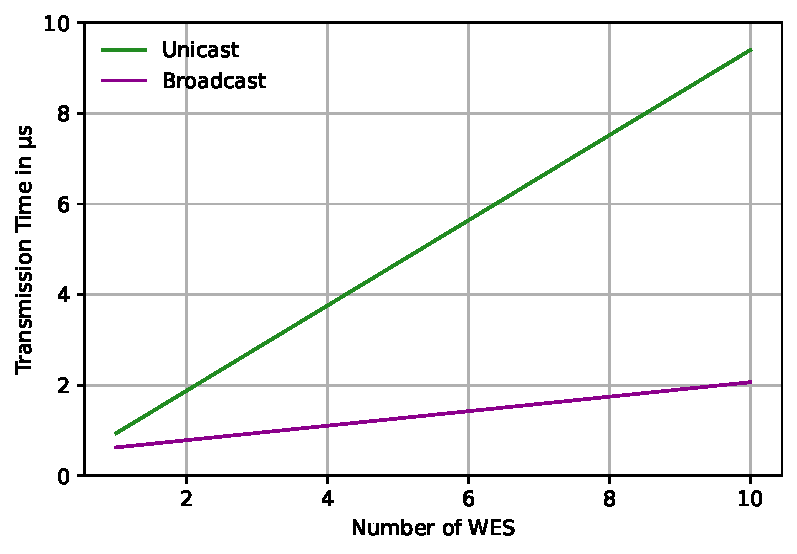
\includegraphics[scale=0.7]{/home/walther/Documents/bachelor/Plot2/Graphs/bc_uc_transmissiontime_analytic.pdf}
	\caption{Transmission Time of Unicast vs Broadcast}
	\label{fig:bc_uc_transmissiontime_analytic}
\end{figure}

\begin{figure}
	\centering
	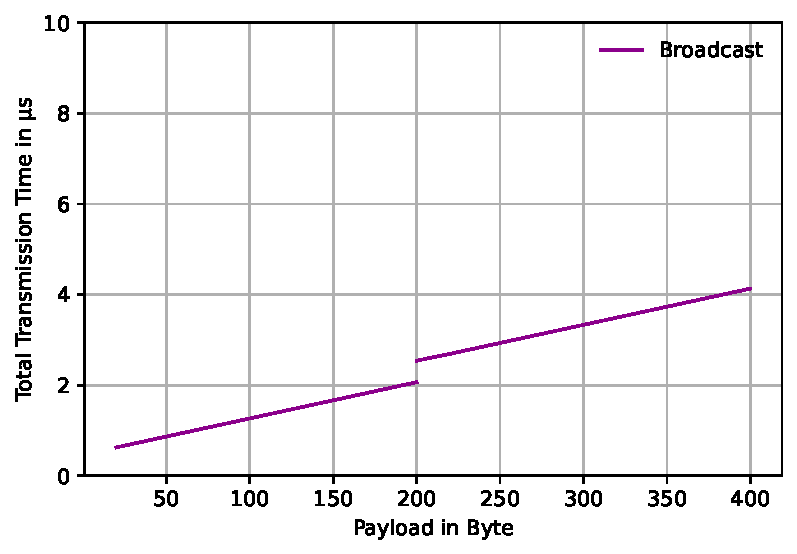
\includegraphics[scale=0.7]{/home/walther/Documents/bachelor/Plot2/Graphs/bc_analytic.pdf}
	\caption{Transmission Time of Unicast vs Broadcast Analytis}
	\label{fig:bc_analytic}
\end{figure}

\subsection{Rapid Repetition}
\begin{itemize}
\item simple
\item redundant
\item fast
\item cite paper from tolja
\item explain why its only relevant for BC?
\end{itemize}

The ESP-Now broadcast does not support acknoledgements.
So we can't retransmit a packet to the fixture, which is not arrived successfully.
In case of broadcast we had to transmit the hole broadcast or an unicast to each fixture wich does not send back the acknoledgement.\\

Since this is very cumbersome to implement, it is a good approach to simply repeat each broadcast. 
\TODO{Cite paper A First Implementation and Evaluation of the IEEE 802.11aa Group Addressed Transmission Service}
This is called rapid repetition. \TODO{Is Rapid Repetition a appropriate name? Unsosliced Repetition is better siehe Paper?}
The idea is, that we can push the reliability wich each redundant retransmission.

The estimated reliability of a fixture with average success ratio (SR) of 83\% without Repetition has to be 83\%.
If we increase the number of Rapid Repetitions (RR) we can roughly estimate:
\begin{align}
	% ER &= 1-SR &\text{Errorrate}\\
	SR_{RR}(RR) &= 1-(1-SR)^{RR+1} 
\end{align}
\todo{RR von 0 beginnen}
\TODO{grafische Darstellung RR=[0,1,2,3,4], für einen guten und einen schlechten Knoten 83\% und 95\%}

\begin{figure}
	\centering
	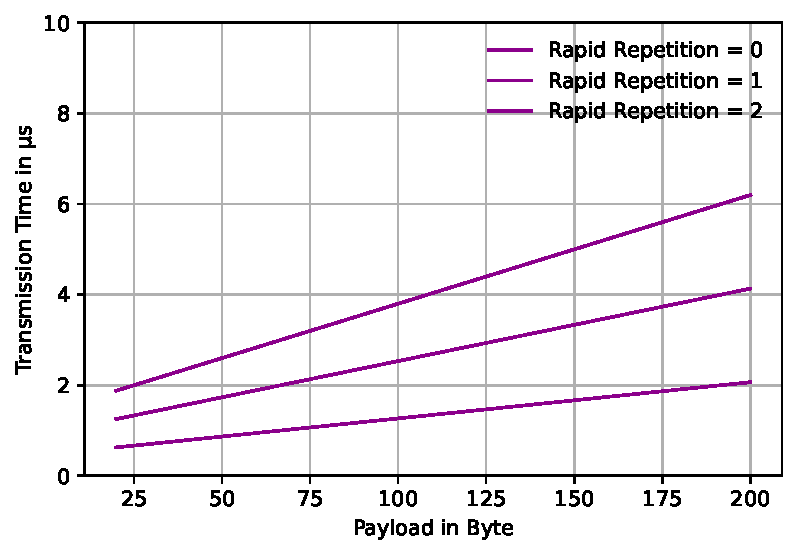
\includegraphics[scale=0.7]{/home/walther/Documents/bachelor/Plot2/Graphs/rr_transmission_time.pdf}
	\caption{Transmission Time with with different \ac{RR}s}
	\label{fig:bc_analytic}
\end{figure}

We have to figure out how many repetitions we should transmit in order to find the best balance between reliability and latency/update ratio.
This hardly correlates with the overall success ratio in the (test-)setup. \TODO{(test-)setup: kann man das so schrieben?}

\subsection{Delayed Repetition}
\label{sub:DelayedRepetition}
\begin{itemize}
\item when to perform repetition
\item buffering delay
\item explain why its only relevant for BC?
\end{itemize}

To push the idea of rapid repetion even further, we should take a look to temporarily occuring disturbances.
\TODO{Figure of bad channel time}

\section{Implementation}
\begin{itemize}
\item ESP programming
\item code examples
\item python script
\end{itemize}

\todo{for later use: ESP-NOW User Guide, V1, source: \url{https://www.espressif.com/en/support/documents/}}

\subsection{ESP Programming}
\begin{itemize}
\item broadcast unicast
\item IDF/Arduino
\item IDE \& ESP hardware flashing
\item setup devices
\end{itemize}
Unfortunally in the documentation of the ESP-protocol is written, that broadcast is not supported 
% \TODO{link, https:\/\/www.espressif.com\/sites\/default\/files\/documentation\/esp-now_user_guide_en.pdf, 2016}
but actually it is. Insted of adding the \ac{MAC} Address of a fixture, we can use 
\todo{has this a proper name, like broadcast address?} ff:ff:ff:ff:ff:ff 
to add a peer with the broadcast \ac{MAC}.

\label{lst:shorttable}
\begin{lstlisting}
void addFixtureToPeerList(const uint8_t *mac_addr) 
{
	if (esp_now_is_peer_exist(mac_addr)) return;

	peer_info.channel = 1;               // 1-14
	peer_info.ifidx   = ESP_IF_WIFI_STA; // Station mode
	peer_info.encrypt = false;         	 // not needed
	memcpy(peer_info.peer_addr, mac_addr, 6);

	esp_err_t status = esp_now_add_fixture(&peer_info);
	if (ESP_OK != status) 
	{
		Serial.println("[ERROR] Could not add fixture");
	}
	else 
	{
		Serial.println("[OK] fixture added");
	}
}
\end{lstlisting}
% \lstinputlisting[caption=Scheduler, style=customc]{hello.c}

\TODO{fix colorscheme omf code examples}

\subsection{Collecting measurment results}
\begin{itemize}
\item Collecting values
\item state machine
\item python script
\item saving values
\item digital encoding e.g.: 777477472717
\end{itemize}

\begin{figure}
	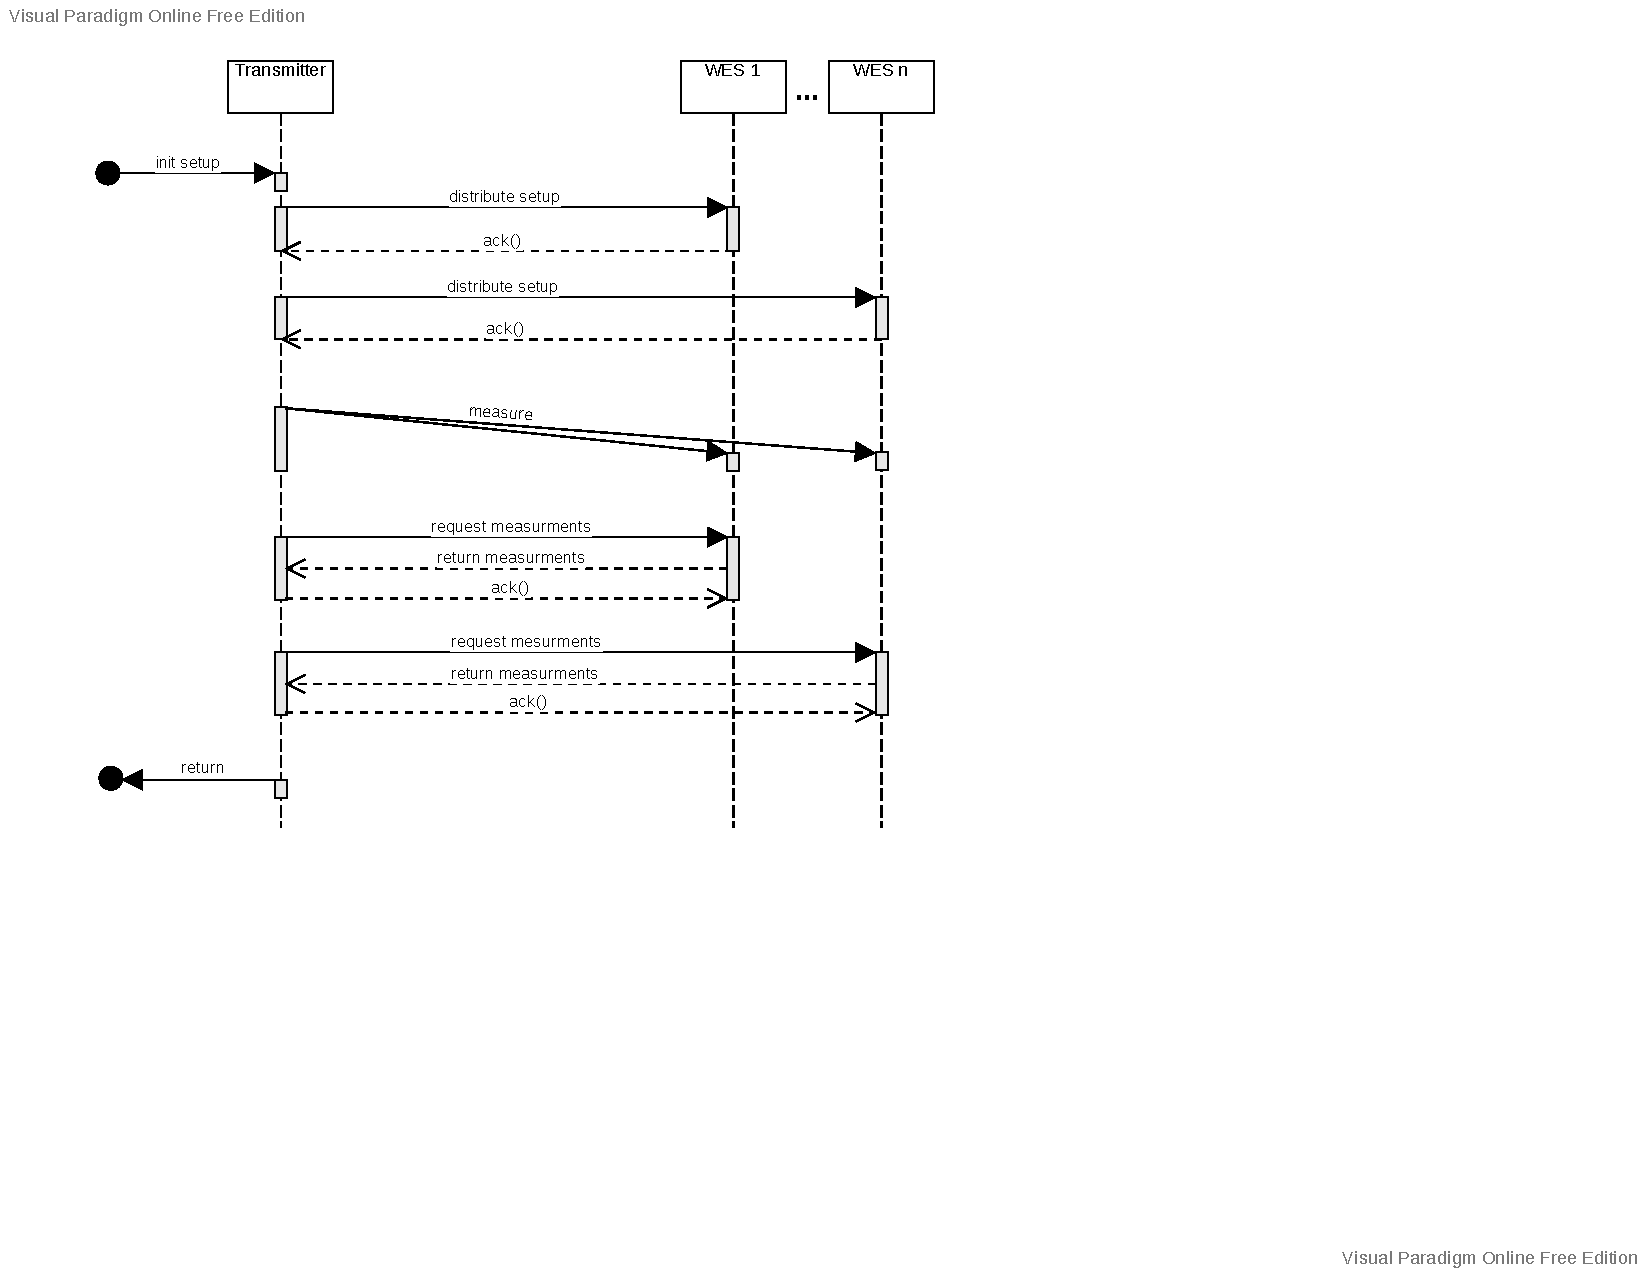
\includegraphics[scale=0.8]{figures/sequence_diagram.pdf}
	\caption{Sequence diagram of the measurment}
	\label{fig:sequenceDiagram}
\end{figure}

\begin{sequencediagram}
	\newinst{c}{:computer}
	\newthread{t}{:Transmitter}
	\newinst[2]{w}{:WES 1}
	\newinst{n}{:WES n}

	% give test vector to transmitter via serial
	% \begin{call}{c}{testVector()}{t}{ack()}
	\mess{c}{Test Parameter}{t}

	% \begin{sdblock}{}{distribute test parameter}
	\begin{call}{t}{Test Parameter}{w}{ack()}
	\end{call}
	\begin{call}{t}{Test Parameter}{n}{ack()}
	\end{call}
	% \end{sdblock}

	\mess[1]{t}{measurments}{w}
	\mess[1]{t}{measurments}{n}	

	\begin{call}{t}{request measurment}{w}{ack()}
	\end{call}
	\begin{call}{t}{request measurment}{n}{ack()}
	\end{call}
	% \begin{call}{t}{function()}{wn}{ack()}
	% \end{call}
	\mess{t}{Test Results}{c}

\end{sequencediagram}

\chapter{Evaluation}
\begin{itemize}
\item measurement setup / results / evaluation / discussion
\item whatever you have done, you must comment it, compare it to other systems, evaluate it
\item usually, adequate graphs help to show the benefits of your approach
\item each result/graph must not only be described, but also discussed (What's the reason for this peak? Why have you observed this effect? What does this tell about your architecture/system/implementation?)
\item recommended length: approximately one third of the thesis.
\end{itemize}

\section*{Keep in Mind}
\begin{itemize}
\item metrics (SR, Latency, ...)
\item compare with art-net all the time
\end{itemize}

\section{Methodic}
\begin{itemize}
	\item Testbed
	\item Collect Data
	\item Seqence Diagram to explain 
\end{itemize}

\section{Protocols under Study}
\begin{itemize}
	\item 
\end{itemize}
\subsection*{Unicast vs Broadcast}
\subsection*{Rapid Repetition}
\subsection*{Delayed Repetition}
\subsection*{Grouping}

\section{Results}
\TODO{Difference between Results and Discussion?}
\begin{itemize}
	\item Grafen miteinander verlgeichen?
	\item Which method had the best results?
\end{itemize}

\chapter{Conclusion \& Discussion}
\begin{itemize}
\item summarize again what your paper did, but now emphasize more the results, and comparisons
\item write conclusions that can be drawn from the results found and the discussion presented in the paper
\item future work (be very brief, explain what, but not much how, do not speculate about results or impact)
\item recommended length: one page.
\end{itemize}

Why not 5GHz -> to expensive.\\

\newcommand{\comment}[1]{}
\comment{
\chapter{Guidelines}

The following are general guidelines for how to write a thesis, with a special focus on how to use the template we provide.
Please read it in full before starting.

This template already includes a large number of LaTeX packages.
Make sure you use an up-to-date LaTeX distribution, such as \emph{TeX Live 2020}.
Familiarize yourself with the available package options of this template (such as the \texttt{germanthesis} and \texttt{watermark} options).


\section{Typesetting}

You can include many non-ASCII characters (like umlauts äöü or accented characters in general ñçø) verbatim in your \texttt{.tex} code, but make sure to save the file using UTF-8 encoding.

Use double quotation marks only for text cited from other work ``like this''.
Use bold text \textbf{very sparingly}, as it is likely to interrupt a reader's flow of reading.
Instead, use the \texttt{emph} command to typeset such text in a \emph{somewhat} less intrusive way (while still indicating a change in the tone of voice).

Use paragraphs to break the content into logical groups.
Do not use hard\\ line breaks. In the source file, however, line breaks have proven to simplify editing considerably: putting exactly one sentence per line makes it very easy to move content around, it helps quickly identifying overly long sentences, and allows line-based diff tools to work as expected.

Consider using the \texttt{textsc} command to make long runs of capital letters slightly less intrusive.
Typesetting PCMCIAPEBKAC as \textsc{Pcmciapebkac} makes the text stand out much less on the page.


\section{Cross References}
\label{sec:cross-ref}

Cross references are an easy way to point a reader to certain parts of the text.
For figures, tables, and equations, they are a must.
Sometimes, it is also useful to point a reader to other sections, e.g., to \cref{sec:cross-ref}, but this should be used sparingly.

\section{Figures}

\begin{figure}%
	\centering
	\subfloat[coverage]{\label{fig:setup1}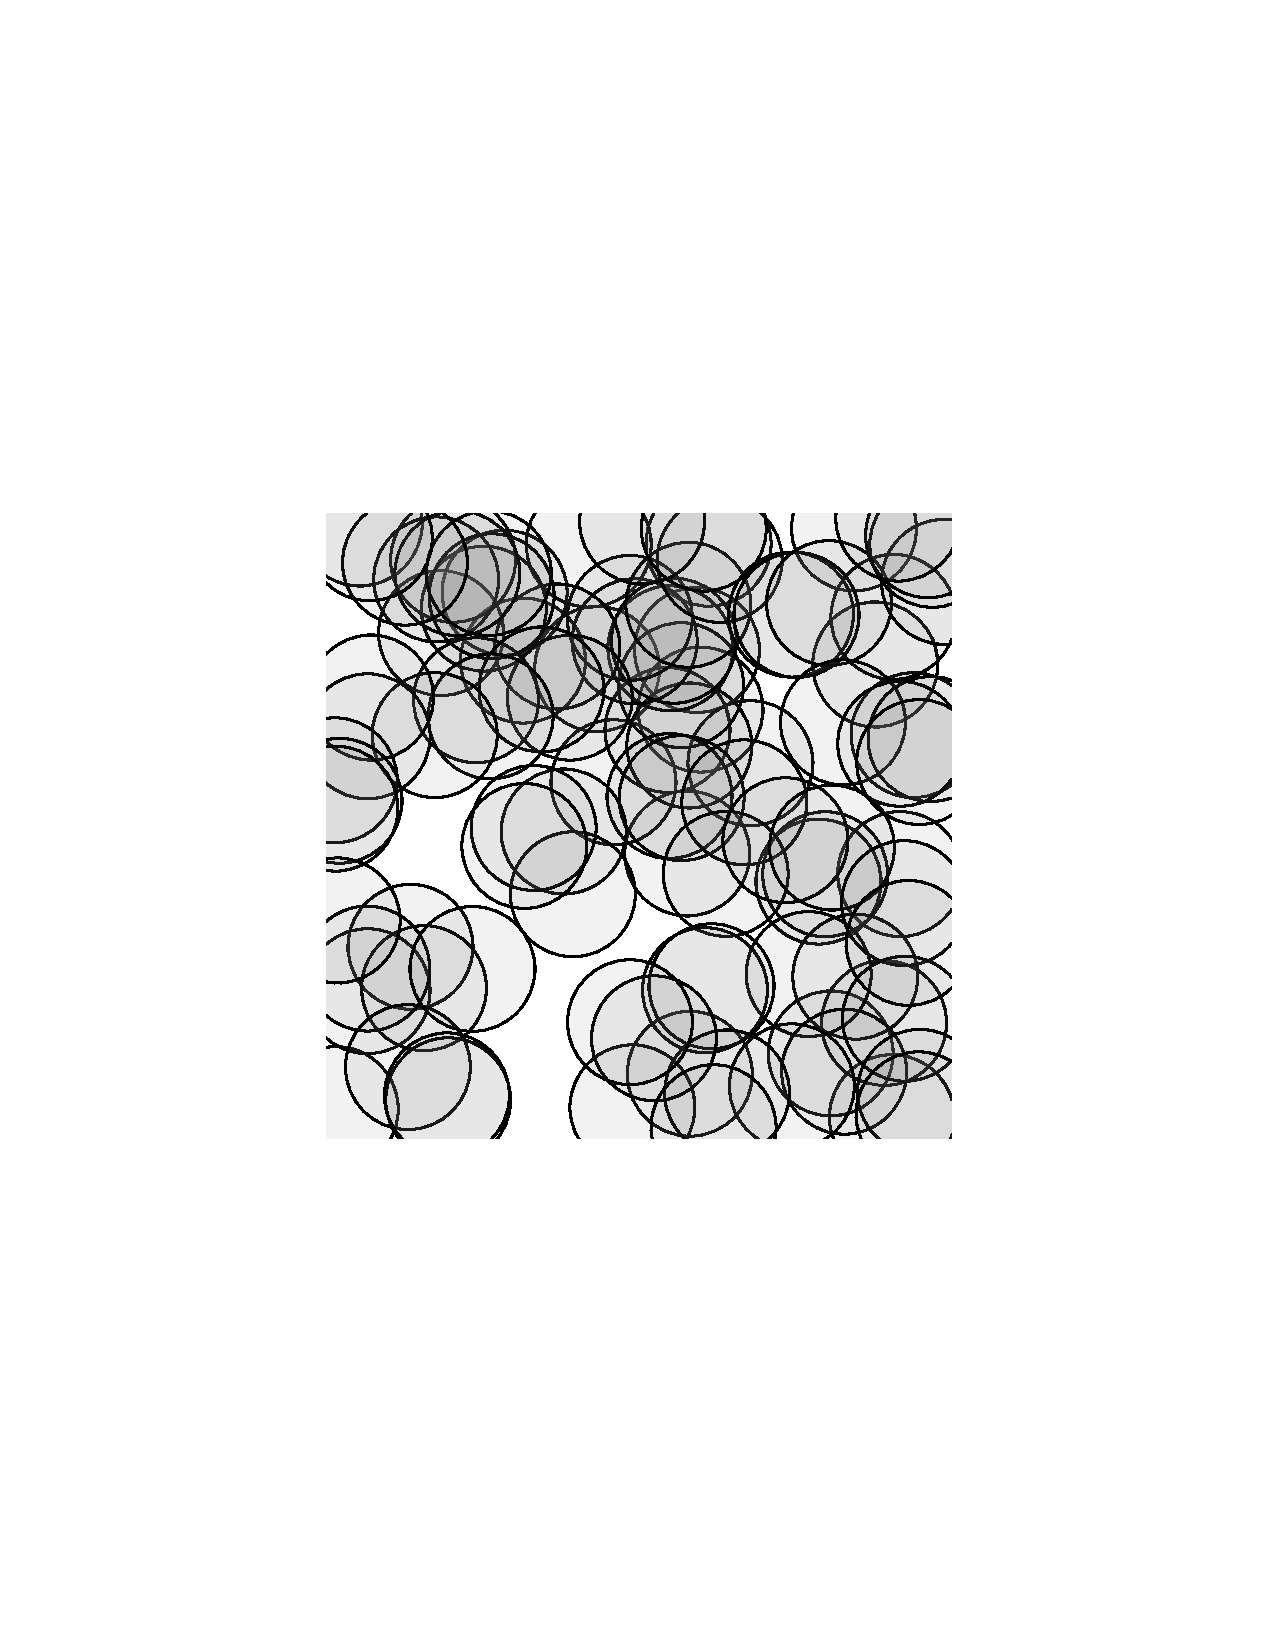
\includegraphics[width=0.3\textwidth]{figures/coverage-30--0-static1}}%
	\subfloat[connectivity]{\label{fig:setup2}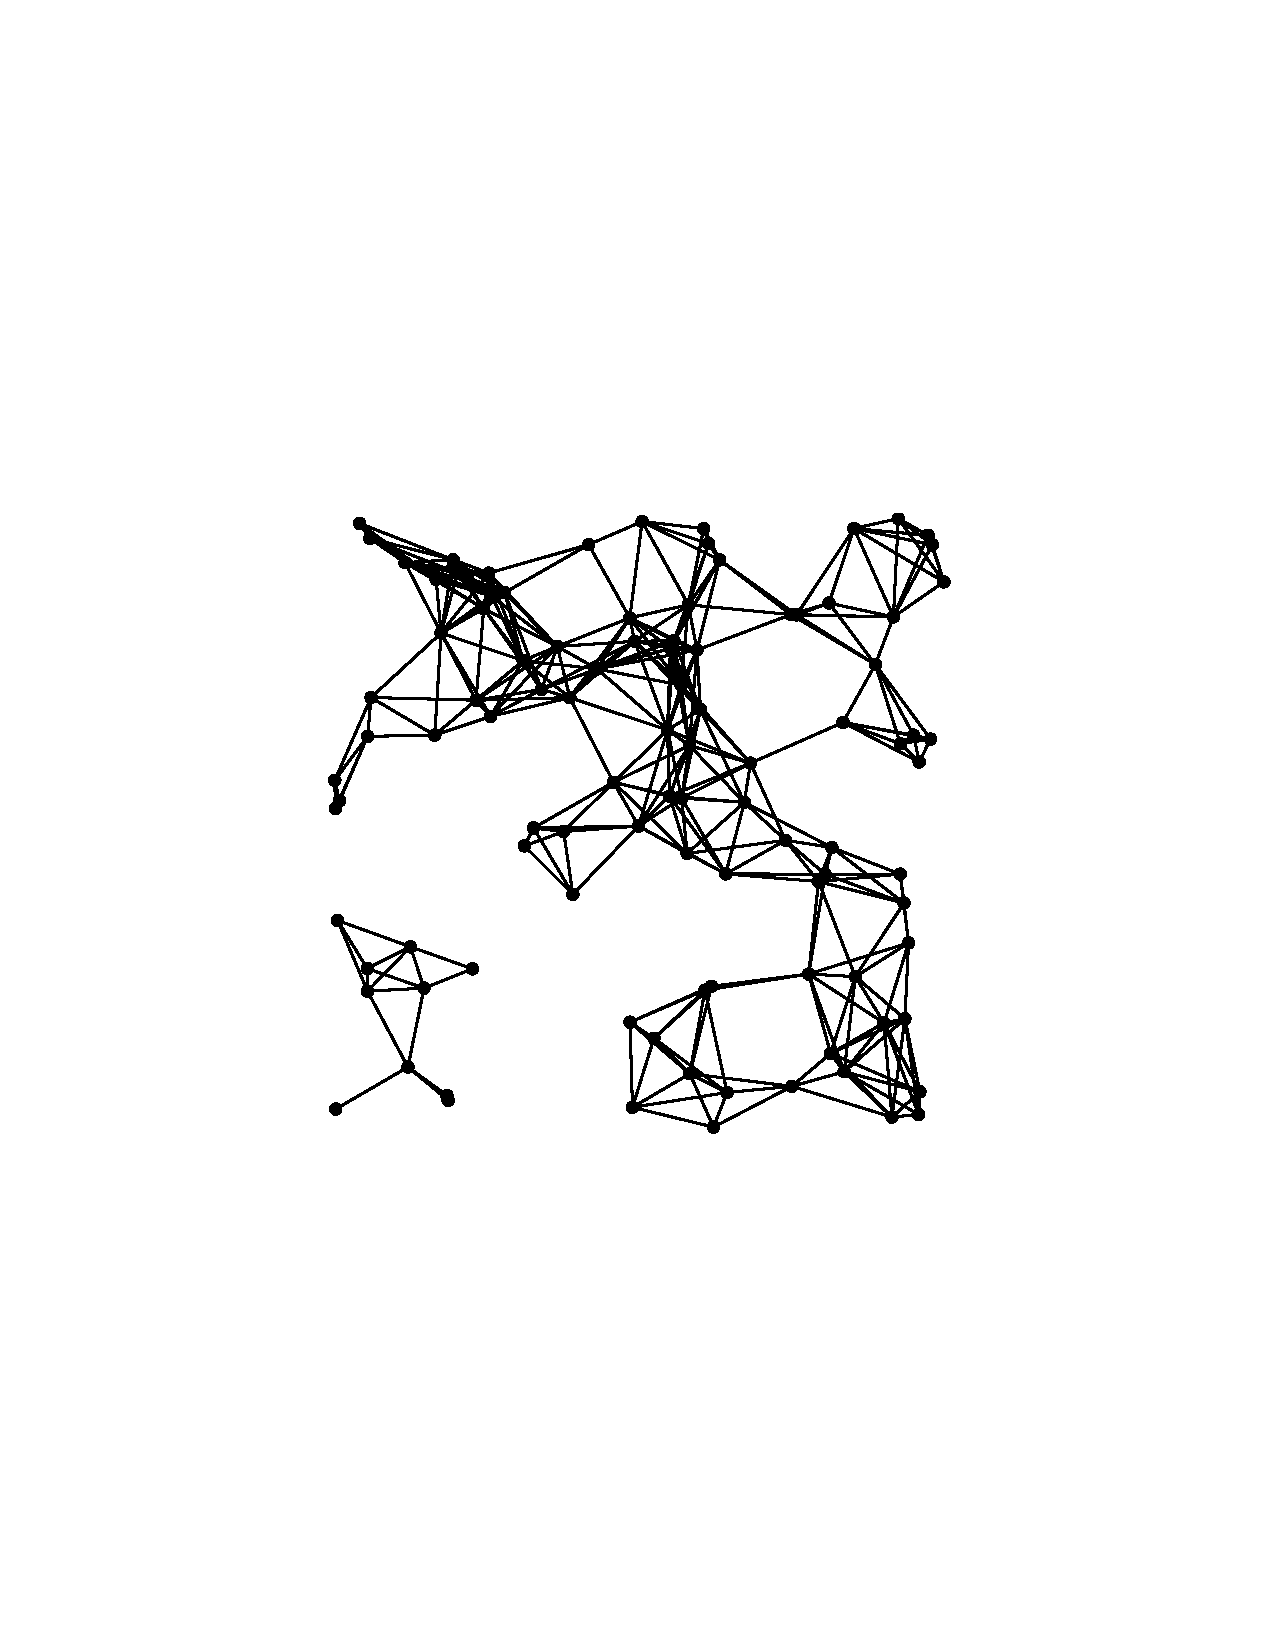
\includegraphics[width=0.3\textwidth]{figures/connectivity-50-0-static1}}
	\caption{Subfigures showing coverage and connectivity for a sample replication at time $t=0$}%
	\label{fig:setups12}%
\end{figure}

A picture says more than a thousand words.
Use \texttt{jpeg} files for photos, use \texttt{png} for screenshots, use \texttt{pdf} for everything else.
Make sure to include all text required to get a (cursory) understanding of the figure in its caption; it is no problem to have a caption spanning five lines.
Do not put a second caption in the figure itself.
For closely related content, consider using subfigures.
Draw figures yourself, but acknowledge all sources.
Check font sizes to make sure the figure is neither unreadably small nor overly big: after typesetting the thesis, text in the figure should be the same size as that in the figure caption.

Example: \cref{fig:setup1,fig:setup2} show the distribution of the nodes in the sample setup at time $t=0$, as well as the initial coverage with a sensing radius of \SI{30}{\metre} and the communication graph for a communication range of \SI{50}{\metre}.

\clearpage
\section{Tables}

\begin{table}
	\centering
	\begin{tabular}{llr}
		\toprule
		left aligned & same here & right aligned \\
		\midrule
		1 & 2 & 3 \\
		4 & 5 & 6 \\
		7 & 8 & 9 \\
		\bottomrule
	\end{tabular}
	\caption{Short table}
	\label{tab:shorttable}
\end{table}

Use short tables, e.g., \cref{tab:shorttable} to give a brief overview of related information.

\begin{table}
	\centering
	\begin{tabular}{>{\raggedright}p{1.7cm}p{5.4cm}p{3.4cm}}
		\toprule
		Class & application examples & lifetime aspects \\
		\midrule
		Critical, coverage &
				Forest fire detection, flood detection, nuclear/chemical/biological attack detection, battlefield surveillance, intrusion detection &
				$c_{ca}$/$c_{ct}$/$c_{cb}$, $c_{ln}$, $c_{la}$, $c_{lo}$\\
		Critical, no coverage &
				Monitoring human physiological data, military monitoring of friendly forces, machine monitoring &
				$c_{cc}$, $c_{ln}$, $c_{la}$, $c_{lo}$ \\
		Noncritical, coverage &
				Agriculture, smart buildings, habitat monitoring (sensors monitor the inhabitants in a region) &
				$c_{ac}$/$c_{tc}$/$c_{bc}$, $c_{cc}$, $c_{sd}$ \\
		Noncritical, no coverage &
				Home automation, habitat monitoring (sensors are attached to animals and monitor their health and social contacts) &
				$c_{cc}$, $c_{sd}$ \\
		\bottomrule
	\end{tabular}
	\caption{Sensor network applications}
	\label{tab:SensorNetworkApplications}
\end{table}

For presenting result data, a figure is much more appropriate.
Multi-line cells can be typeset as shown in \cref{tab:SensorNetworkApplications}.

\clearpage
\section{Math}

Equations are frequently referred to by other papers.
Make sure that they are broken up into logical groups and that each of your equations is numbered.
Use in-line equations for very simple statements only.
To give an example, $\zeta(t) = \min( \zeta_{**}(t))$ is much better written as
\begin{equation}\label{eq:zeta}
\zeta(t) =
	\min\left(
		\zeta_{**}(t)
	\right)
,
\end{equation}
which is also easier to find.

Equations covering multiple lines should be aligned.
Note that the numbering is (and should be) added, independent of whether the equation is actually referenced or not, as in
\begin{align}
sd_{max} &=
	\max\left(
		(t_{i+1} - t_i)
			: \zeta(t_i) < 1, i \in [0, |T|-1]
	\right)
,\\
\psi_{sd}(t) &=
	\begin{cases}
		\dfrac{\Delta t_{sd}}{sd_{max}}
			& \text{if $sd_{max} > 0$}, \\
		1
			& \text{if $sd_{max} = 0$},
	\end{cases}
\\
\zeta_{sd}(t) &= 
	\frac{
		\psi_{sd} - cl_{sd}
	}{
		c_{sd} - cl_{sd}
	}
.
\end{align}

The \emph{User's Guide for the amsmath Package}\footnote{\url{http://mirrors.ctan.org/macros/latex/required/amslatex/math/amsldoc.pdf}}, provided by the American Mathematical Society, has a comprehensive overview of best practices for typesetting mathematical content.


\clearpage
\section{Units}

Numbers with units should be set using the \verb|\SI| command, which enforces consistency throughout the text.
For example, the measurements show that the car was accelerating at \SI{5}{\metre\per\second\squared} until it reached its final speed of \SI{100}{\kilo\metre\per\hour}.

Units without a number can be typeset using \verb|\si|; longer unit-less numbers or ranges can be typeset using the \verb|\num| and \verb|\numrange| commands, respectively: The number \num{12345678} lies in the range of \numrange{10000000}{20000000}.
\Cref{tab:si-in-tables} gives an example of how to typeset numbers and units in tables.

Here I deleted a Algorithm example. I hope that i wont need it again.

\clearpage
\section{Algorithms}

Use algorithms to explain what would be too hard to express in the text body of your thesis.

For example: Based on the periodically transmitted \texttt{hello} messages, the joining node gets information about its physical neighbors and their adjacent nodes.
\Cref{alg:H_hello} depicts the handling of \texttt{hello} messages.

\begin{algorithm}
\begin{algorithmic}[1]
\REQUIRE Locally stored state of all neighbors in set $N$
\ENSURE Maintain neighbor set $N$ and set virtual address
\STATE Receive neighbor information from node $N_i$
\IF {$N_i \notin N$}
	\STATE $N \gets N_i$
\ELSE
	\STATE Update $N_i \in N$
\ENDIF
\IF {$P==-1$ AND (Time() $-$ OldTime) $> T_{ps}$}
	\STATE OldTime $\gets$ Time()
	\STATE SetMyPosition()
\ENDIF
\end{algorithmic}
\caption{Handle \texttt{hello} messages}
\label{alg:H_hello}
\end{algorithm}

\clearpage
\section{Typesetting Grammars}

Grammars can be typeset using the \texttt{grammar} environment.

\begin{grammar}\label{stx:demo}

<input> ::= <primary> `;' <input> \alt <primary> \alt \empty

<primary> ::= <term> | "NUMBER"

<term> ::= <primary> <operator> <primary>

<operator> ::= `*' | `/'

\end{grammar}

An alternative graphical form is also available.
This version is often easier to read, but does not lend itself well to more complex grammars.


\clearpage
\section{Program Code}

Program code should be omitted.
What your programs do will already be explained in text form or, if needed, in algorithmic form.
If including source code is absolutely necessary, it should be typeset as seen in ....

\clearpage
\section{References}

What follows is just a very quick refresher on how to use references.
It is not a guide on scientific writing in general, nor copyright and plagiarism in particular.
Please refer to an actual guide on technical writing and scientific practices to make sure you understand how, where, and when to cite.

Simply speaking, proper scientific writing has to deal with two closely related (but not identical) concepts:
\begin{enumerate}[label=\alph*),ref=(\alph*)]
\item\label{itm:ref:copy}
Copyright
\item
Plagiarism\label{itm:ref:plag}
\end{enumerate}
Do not confuse the need for properly citing your sources as something related to copyright.
Questions of~\ref{itm:ref:copy} copyright or the corresponding national equivalent deal with who has the right to reproduce a certain text excerpt, an image, or something similar.
Questions of~\ref{itm:ref:plag} plagiarism deal with who came up with a certain idea or insight, e.g., a certain finding, a certain concept, or a certain way of illustrating a concept.
By way of analogy, consider a car: after buying a car you have the right to~\ref{itm:ref:copy} do whatever you want with it, but you still cannot claim that you~\ref{itm:ref:plag} invented it.
Conversely, properly~\ref{itm:ref:plag} crediting who invented your neighbor's car does not give you the right to~\ref{itm:ref:copy} use it.
Put yet another way, problem~\ref{itm:ref:copy} is a legal one: to be allowed to publish a scientific work you (or, rather, your publisher) needs to have permission to reproduce it -- or suffer legal consequences like heavy fines.
Problem~\ref{itm:ref:plag} is an academic one: claiming someone else's ideas as one's own is plagiarism; similarly, re-selling old ideas as new ones is self-plagiarism.
Both incur heavy penalties like exclusion from schools and professional associations or being blacklisted from publishing with scientific outlets for any number of years.

You will need to address both problems in writing your thesis.
Problem~\ref{itm:ref:copy} can be addressed in two ways:
First, by creating original content (that is, text or figures) yourself, which is always preferable as this gives you the freedom to present the content your way.
Second, by obtaining a license to reproduce content (e.g., by way of buying a license or adhering to the terms of an existing copyleft license).
Problem~\ref{itm:ref:plag} can be addressed in two ways:
First, presenting original ideas and insights (as you will do when presenting own results).
Second, by clearly pointing out the (primary) source of an idea.
The latter is the topic of this section.

In brief, use references whenever you cite from related work (either directly or indirectly), or when you build on related work (this includes their way of illustrating a particular concepts, in text form as well as in the overall design of a figure).
Also use references to point a reader to related work.
Clearly distinguish between these uses.
Make it very clear which part of a statement a reference belongs to.
Compare the following three, vastly different uses (where the cited idea appears in \textbf{boldface}):

\begin{itemize}
\item ``\textbf{Foo and bar are of equal value. Thus, any can be used.}''~\cite{akyildiz2002survey,arampatzis2005survey}
\item According to~\cite{akyildiz2002survey} and~\cite{arampatzis2005survey}, \textbf{foo and bar are of equal value, and any can be used}.
\end{itemize}
versus
\begin{itemize}
\item ``\textbf{Foo and bar are of equal value}''~\cite{akyildiz2002survey,arampatzis2005survey}. Thus, any can be used.
\item According to~\cite{akyildiz2002survey} and~\cite{arampatzis2005survey}, \textbf{foo and bar are of equal value}. From this it follows that any can be used.
\end{itemize}
versus
\begin{itemize}
\item Foo and \textbf{bar}~\cite{akyildiz2002survey,arampatzis2005survey} are of equal value. Thus, any can be used.
\item Foo and \textbf{bar} (detailed in~\cite{akyildiz2002survey} and~\cite{arampatzis2005survey}) are of equal value. Thus, any can be used.
\end{itemize}
versus
\begin{itemize}
\item \textbf{Foo}~\cite{akyildiz2002survey} and \textbf{bar}~\cite{arampatzis2005survey} are of equal value. Thus, any can be used.
\item \textbf{Foo} (detailed in~\cite{akyildiz2002survey}) and \textbf{bar} (detailed in~\cite{arampatzis2005survey}) are of equal value. Thus, any can be used.
\end{itemize}

Never typeset a reference after the final full stop of a paragraph (or sentence) and expect your reader to figure out which part of the paragraph is an indirect citation and which part is original (i.e., your own) work.
When paraphrasing longer passages of text, use an indirect citation.
Make sure to clearly point out when you are finished paraphrasing, like so:
\emph{According to \textcite{akyildiz2002survey}, Foo and Bar can be characterized as follows. They are big. They are bright. The authors further argue that one can be substituted for the other. In the following I will go on to prove that this is not true.}

When citing more than a few pages worth of text, point the reader to the specific part you are referring to in your citation, like so:
\emph{In recent years, an increasing number of cyclists are switching from air filled tires to cement filled ones~\cite[Table IV]{dietrich2009lifetime}}.

If a figure or a table is closely based on another one, make sure to cite its source, preferably in its caption, like so:
\emph{Figure 1 -- the relation of ravens and writing desks (based on~\cite[Figure~42]{dietrich2009lifetime})}.
Be aware that, while there is a well-established convention on how to illustrate a verbatim quote of text (by using quotation marks), there is no well-established convention for indicating that an image was copied verbatim.
Thus, when citing a figure or table, you must explicitly state whether it was copied verbatim, ed, or whether it served as inspiration for your own.

Do not cite URLs. Content found there is not peer reviewed and it is likely to change during the lifetime of your work.
For pointing a reader to interesting websites, use footnotes -- but trust your reader to know how to use a web search engine.

Your text reads nicer if you do not use citations as a substitute for nouns (like this section did).
Instead of \emph{The benefits of cement filled tires has been shown by \cite{akyildiz2002survey}}, consider writing \emph{\textcite{akyildiz2002survey} have shown the benefits of cement filled tires}.
The \texttt{textcite} command makes this straightforward.

Make sure to read your bibliography section (that is, the typeset list of references) after you are done adding all citations to your text.
Does it contain all information needed to uniquely identify to references you used?
Do not trust BibTeX files you find on the web:
Digital libraries frequently have their contents wrong, are missing information, or are using different field names than your bibliography style expects (leading to missing information in the typeset bibliography).
To give a few examples:
Check the authors' list (making sure all authors are listed in the same order and in the same way they are listed in the publication).
Check the conference location (it's most likely not ``New York, New York'').
Check the publisher name (many digital libraries use a field that is not typeset by your bibliography style; have a look at the demo bibliography in this template for how to deal with that).
Check the page numbers (many digital libraries put ``1--5'' here despite the paper starting at a later page -- or despite it not having any page numbers to begin with).
Check the conference name, put its parts in a logical order, and lose the ``in proceedings of'' (it's not ``Mobicom, in proceedings of, 1999 series MobiCom99'' but ``5th ACM International Conference on Mobile Computing and Networking (MobiCom 1999)''.\todo{triple-check all references}


\section{Abbreviations}

Abbreviations should be explained when first used.
Latex helps by providing an \verb|\ac| command that will automatically expand an abbreviation on first use.

\begin{description}

\item[first use:]
\acp{MANET} have been frequently used as examples for the development of \ac{WSN} applications.
Simulations are made more efficient by the use of \iac{ROI}.

\item[second use:]
\acp{MANET} have been frequently used as examples for the development of \ac{WSN} applications.
Simulations are made more efficient by the use of \iac{ROI}.

\end{description}

Make sure to explicitly choose either the short \verb|\acs*|, long \verb|\acl*|, or full \verb|\acf*| starred form in headings and captions to avoid unpleasant surprises.

Automatic abbreviations also support ones that only make sense in a foreign language -- like that of the \ac{ADAC}.
Some care must be taken when the same abbreviation can refer to multiple things -- like \ac{CANproto} and \ac{CANhashing}.

In general, use (explained) abbreviations sparingly:
Your reader can be assumed to know what a MAC is, what UMTS or GPS do, etc (and, if not, spelling these terms out won't be of much help, anyway).
Further, each newly introduced abbreviation increases your reader's cognitive load (you are expecting your reader to be able to recall any of your introduced abbreviations at any later point in the text).


\section{TODOs and FIXMEs}

You can use the the \verb|\TODO| command to add short ``sticky notes'' to your document.
\TODO{This is what a TODO looks like}
This will also trigger generation of a list-of-TODOs at the end of the document.
The same goes for the \verb|\FIXME|\FIXME{This is what a FIXME looks like} command.


\section{Sections}

Keep the number of sections and sub-sections low.
If two sections start on the same page, you are most likely using too many sections.
Each section should include some text (i.e., the heading of section~1 should not be immediately followed by the heading of section~1.1)

Stay clear of \emph{meta} writing, that is, explicitly addressing the way your thesis is laid out:
Rather than ``this section contains two sub-sections'', say ``in the following, I will address two important results: foo and bar''.

Do not use section headings as a replacement for introductory text and a short motivation.
It should be easy enough to follow your thesis with all section headings removed.

\section{About the remainder of this document}
The remainder of this document gives a rough outline of how to structure your thesis.
It is mainly geared towards Bachelor and Master's theses, but feel free to adapt the structure to your specific needs.
If, however, you are writing a seminar thesis, the present structure is likely wholly inapplicable.
}

\cleardoublepage

\listofabbreviations
\clearpage

\listoffigures
\clearpage

\listoftables
\clearpage

\printbibliography

\end{document}
